\documentclass[../Main.tex]{subfiles}

\begin{document}
\author{Wave-Particle Duality} %use author for title of lesson
\date{Year 1 Topic 21} %use date to refer to topic in main booklet

\section{Wave-Particle Duality} %Section is the title of the lesson repeated, ready for the main contents page.

\begin{frame}{Wave \& Particle Nature of Light}
    Light shows behaviours of being a wave and a particle. What evidence is there that light is a wave?
\begin{figure}
\begin{subfigure}
    \centering
    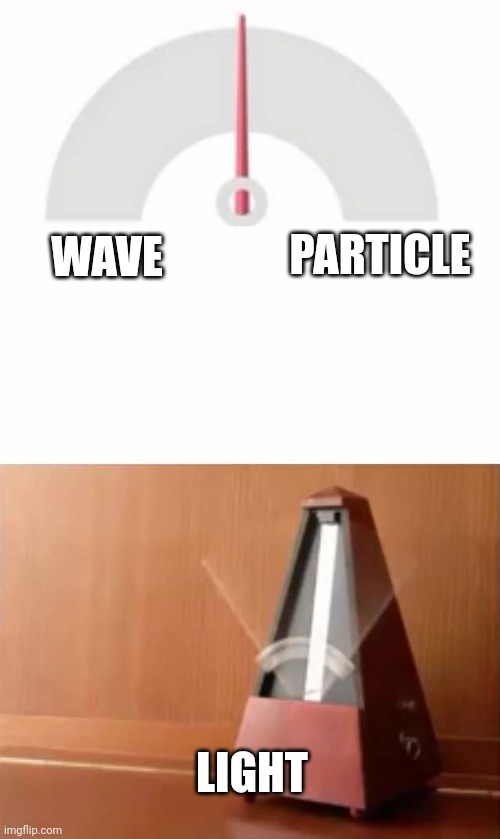
\includegraphics[height=5cm]{Quantum_Images/lightwaveparticle.jpg}
    \end{subfigure} \pause
    \begin{subfigure}
        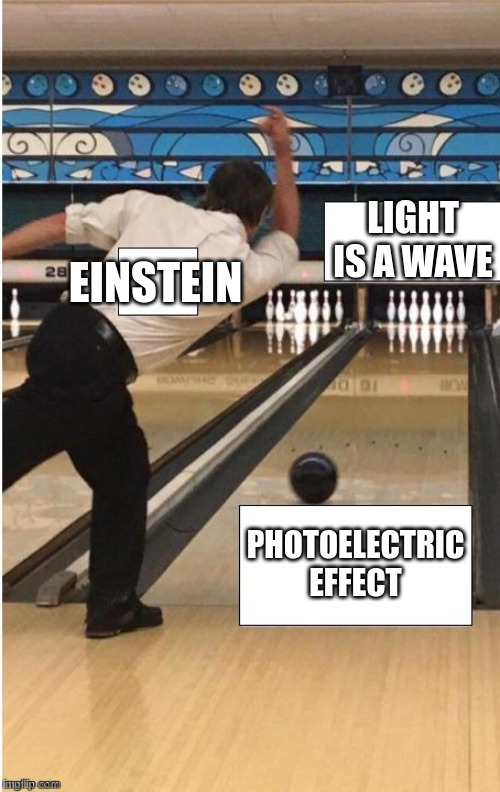
\includegraphics[height=5cm]{Quantum_Images/einsteinbowlingmeme.png}
    \end{subfigure}
\end{figure}
    How do we know light can be a particle?
    -- i.e what do we know about the photoelectric effect?
\end{frame}

\begin{frame}{It's not just light}
    In 1924 Louis de Broglie (pronounced ``der broy'') proposed that it was not just light that, as a particle, could have wavelike properties also. If this were true then particles (e.g. electrons) fired at a double slit and detected on a screen would show an interference pattern. By 1927 an experiment was performed that demonstrated this. 
    
    \begin{figure}
        \centering
        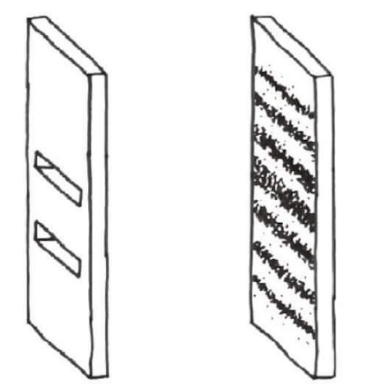
\includegraphics[height=3.5cm]{Quantum_Images/electron_as_wave.png}
    \end{figure}
    
    When streams of electrons were fired at a double slit, a detector in place of a screen detecting where electrons fell showed the appearance of an interference pattern. This suggested that a stream of electrons fired at a double slit interfered with itself -- just like light would.
\end{frame}

\begin{frame}{Electron Interference}
    It was repeated firing single electrons at the screen, slowly building up to show an interference pattern. This showed that even a single electron alone could be a wave that can interfere with itself, suggesting that the electron must be able to be in two places at once! \pause
    
    \begin{figure}
        \centering
        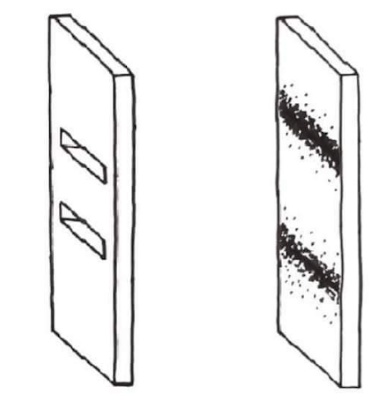
\includegraphics[height=3.5cm]{Quantum_Images/electron_as_particle.png}
    \end{figure}
    But, when a detector was placed at the slit that observed which slit the electron passed through, the interference pattern did not exist. Instead, the ordinary particle behaviour showed.
\end{frame}
    
    \begin{frame}{Wave-particle Duality}
        At the core of quantum physics is the idea that particles can act as both waves and particles -- known as wave-particle duality.
        
        \begin{figure}
            \centering
            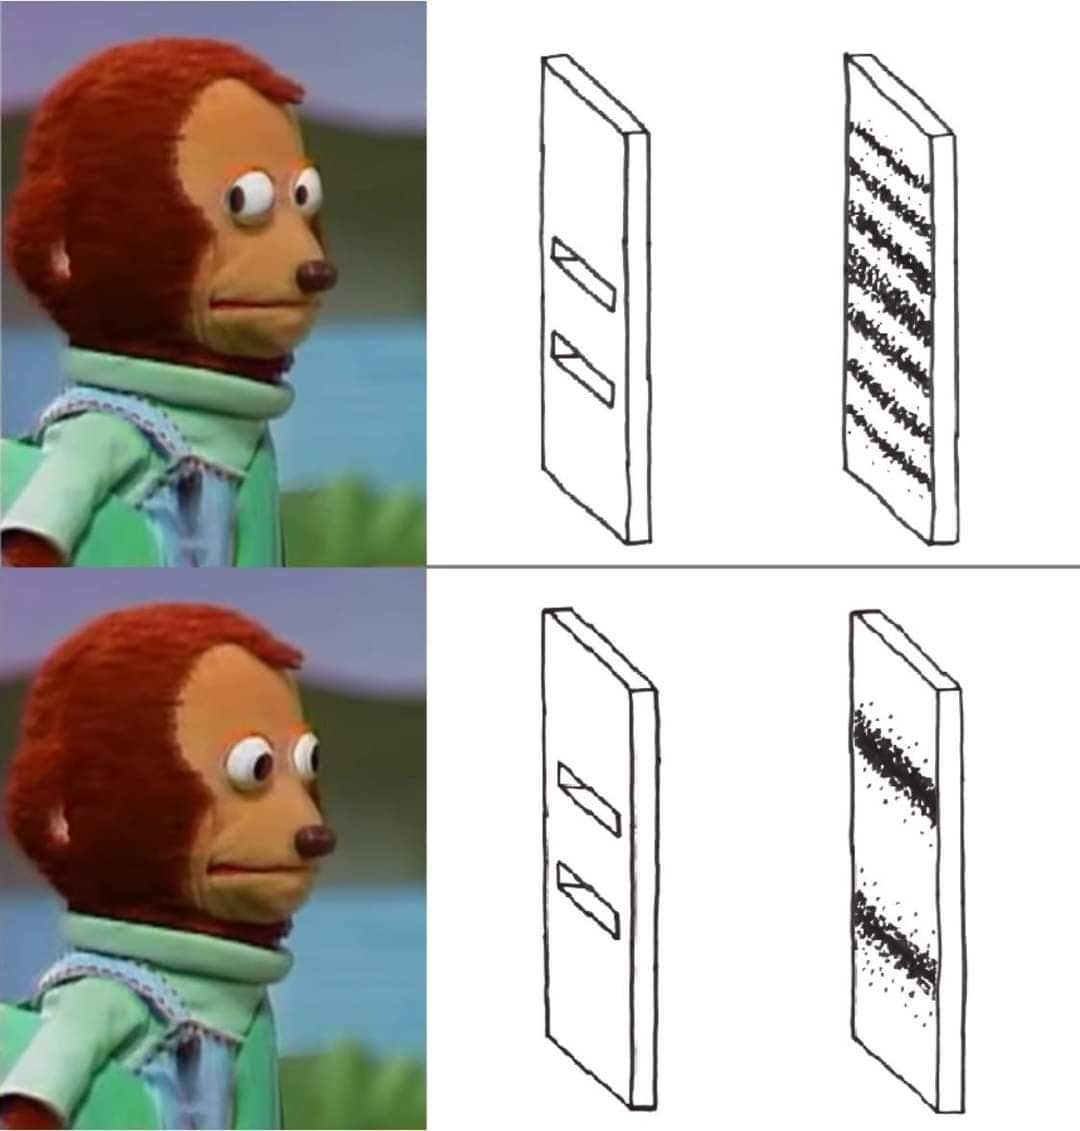
\includegraphics[height=5cm]{Quantum_Images/particlesobserved.png}
        \end{figure}
        It does not have to be a simple electron, all particles have this property -- the largest verified being the C_{60} buckyball
    \end{frame}
    
    \begin{frame}{The Wavelength of Particles}
        de Broglie worked out that the wavelength $\lambda$ of a particle, is inversely proportional to the momentum of the particle. 
        \begin{equation*}
            \lambda \propto \frac{1}{p}
        \end{equation*} \pause
        Through experimentation it was determined that the constant of proportionality is in fact the Planck Constant. Due to his work, the wavelength of a particle became known as the particle's \emph{de Broglie wavelength.}
        \begin{equation*}
            \lambda = \frac{h}{p} = \frac{h}{mv}
        \end{equation*} -- unconvinced? Try to determine the SI unit for $\frac{h}{p}$!
    \end{frame}
    
    \begin{frame}{Examples}
        \begin{exampleblock}{Example 1}
            Calculate the de Broglie wavelength of a proton that has momentum $1.6\times 10^{-19}$kgms$^{-1}$. \pause
            --$4.1\times 10^{-15}m$
        \end{exampleblock} \pause
        
        \begin{exampleblock}{Example 2}
            Calculate the speed of a carbon atom of mass $2.0\times10^{–26}$ kg travelling in space with a de Broglie wavelength of $6.8 \times 10^{–11}$ m. \pause
            --$490ms^{-1}$
        \end{exampleblock}
        \pause
        --Now have a go at some Kerboodle questions, page 253.
    \end{frame}
    
    \begin{frame}{So why is this useful?}
        Note that the information on why this is useful is beyond what you need to know, but that could meet at University if you pursue a Physics-based course.
        
        \begin{block}{Electron Microscope}
            Atoms are significantly smaller than light, so we cannot use light to view an atom. Instead, electrons have a de Broglie wavelength similar to the size of an atom so we can use this to analyse atomic structures
            \begin{figure}
                \centering
                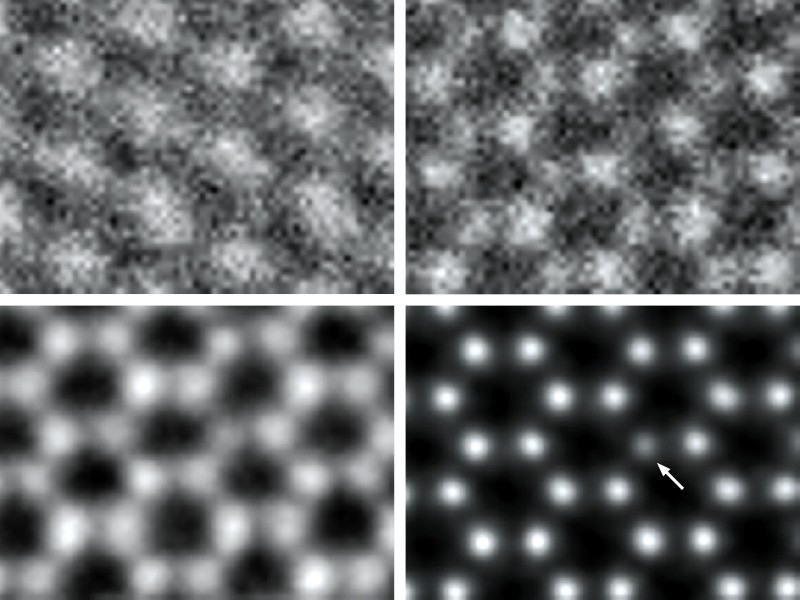
\includegraphics[height=3cm]{Quantum_Images/graphene.jpg}
            \end{figure}
            Each dot in the last image is a carbon atom!
        \end{block}
    \end{frame}
    
    \begin{frame}{So why is this useful?}
        Note that the information on why this is useful is beyond what you need to know, but that could meet at University if you pursue a Physics-based course.
        
        \begin{block}{Quantum Computers}
        Quantum computers use the principle that electrons are a wave, and can act as if in multiple locations simultaneously to perform superfast calculations -- as much as 100 million times faster than an ordinary computer -- imagine the games you could play on that!
            \begin{figure}
                \centering
                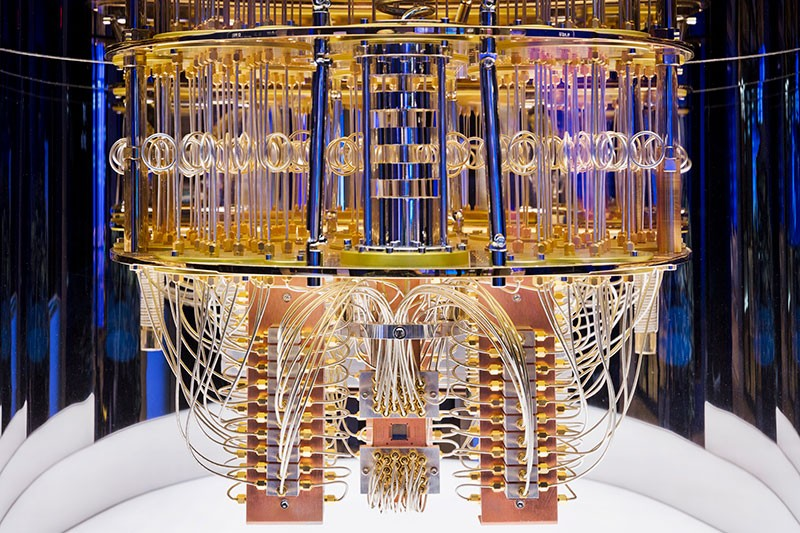
\includegraphics[height=3cm]{Quantum_Images/quantumcomputer.jpg}
            \end{figure}
        \end{block}
    \end{frame}

\end{document}